This chapter describes \sys's high-level semantics that a developer can use to
reason about the resulting state of data after a disguise and reveal, and 
includes an overview of \sys's API.

\section{Disguising and Revealing}
\label{s:semantics:hl}
Developers can think about disguising transformations as removing and rewriting
data in the application database.
%
The database starts at some original application state, and alters application
data depending on the disguise specification (\S\ref{s:semantics:spec}).  The
resulting state---the disguised data state---is changed only by another
disguise, by revealing the applied disguise, or by normal application updates.
%

%
Disguising already-disguised data can only decrease the amount of information
retained about the original application data state. If prior disguises have
transformed the original data, then a future disguise has access only to the
resulting disguised state, and thus can only further remove aspects of the
original data state.
%
Removed data cannot be disguised again. 
%

Disguises may insert pseudoprincipals (anonymous users) into the application
database if the disguise's specification includes a decorrelation, which
rewrites references to point to an anonymous pseudoprincipal instead of the
original principal user. 
%
Same-table data disguised within the same disguise that originally refers to the
same user may decorrelate and refer to the same pseudoprincipal.
%
For example, all decorrelated stories from topic ``Star Wars'' written by Bea
may decorrelate to the same pseudoprincipal (\S\ref{s:semantics:example}).
%
However, no two objects referring to different users or from different database
tables refer to the same pseudoprincipal, and no two disguises' sets of produced
pseudoprincipals overlap.
%

%
\sys applies disguises on behalf of either a single user or all users. However,
only a user can reveal a disguise on their data, and must provide a reveal
credential to do so.
%

%
Revealing a disguise $D$ on some data disguised by $D$ reverts the changes to
the data applied by $D$ back to the pre-disguised state, except in two cases.
First, if a normal application update has since changed the disguised data, then
the data remains in its updated state and cannot be revealed.
%
Second, if another disguise has since applied changes to the data $D$ disguised,
and that disguise has not yet been revealed, then the data remains in its
current state.
%
Only when all subsequent disguises are revealed does the data revert to the
state prior to $D$.
%
Thus, when multiple disguises apply to the same data, the application data state
reflects the effects of all yet-unrevealed disguises.
%

Revealed data will also reflect all global database updates (such as schema
migrations) registered by the developer since the time of disguise, applied in
chronological order.


\paragraph{\sys without encryption.}
\label{s:semantics:noencrypt}

Developers may find \sys's threat model unnecessarily strong: perhaps they do
not worry about data breaches, are exempt from regulations like the GDPR, or
trust their application code to not expose disguised data. Instead, these
developers may want to add disguising and revealing without encryption.
%
Removing encryption does not change \sys's disguising and revealing semantics
described above.
However, because the application and \sys can still see plaintext disguised
data, a user must now trust the application to reveal their data only when 
requested. 
%
\S\ref{s:noencrypt-api} describes how removing encryption would change \sys's
API, and \S\ref{s:noencrypt} describes how it would change
\sys's design.


%%%%%%%%%%%%%%%%%%%%%%%%%%%%%%%%%%%%%%%%%%%%%%%%%%%%%%%%%%%%%%%%%%%
\section{API}
\label{s:api}

\begin{figure}[t]
\begin{lstlisting}[style=rust,escapeinside={(*}{*)}]
// Registers u for disguising and returns u's reveal credentials 
(*\textbf{RegisterPrincipal}*)(
        u: UID, 
        pw: Password,
        pubkey: Option<PublicKey>, 
        privkey: Option<PrivKey>)
    -> RevealCredential;

// Disguises data according to the spec, optionally only for user u, 
// and optionally over already-disguised data ((*\S\ref{s:composition}*))
(*\textbf{DisguiseData}*)(
        u_opt: Option<UID>, 
        spec: DisguiseSpec,
        principal_gen: PrincipalGenerator,
        schema: Schema,
        disguise_over: Option<RevealCredential>) 
    -> disguiseID;

// Reveals data disguised by d for u with u's username password. 
(*\textbf{RevealData}*)(
        u: UID, 
        cred: RevealCredential,
        d: disguiseID, 
        pp_ref_policy: PseudoprincipalReferencePolicy,
        allow_partial_row_reveal: bool,
        schema: Schema)
    -> bool;

// Gets principals that u can speak-for.
(*\textbf{CanSpeakFor}*)(u: UID, cred: RevealCredential) -> Vec<UID>;

// Records a reveal-time update spec in the replay log.
(*\textbf{RecordUpdate}*)(update_spec: RevealTimeUpdateSpec) -> bool;
\end{lstlisting}
\caption{\sys's API (Rust-like syntax).}
\label{f:api-high}
\end{figure}
%

Developers add disguising and revealing to their application via \sys's API,
which consists of the functions shown in Figure~\ref{f:api-high}. This section
describes each function and how developers would use them to support disguising
and revealing.

\subsection{\texttt{RegisterPrincipal}}
    \texttt{RegisterPrincipal} registers an application user as a principal
    whose data can be disguised and revealed. Unique users should not be
    registered multiple times. Once registered, data of an undeleted user that
    exists in the database can always be disguised and revealed.  Users deleted
    by a disguise do not need to reregister if revealed.

    \texttt{RegisterPrincipal} returns backup reveal credentials that the
    application should return to the user client.

    \begin{center}
    \begin{longtable}{|m{0.13\textwidth}|m{0.8\textwidth}|}
        \hline
        \textbf{Argument} & \textbf{Description} \\
        \hline
        \texttt{u} & the user's unique identifier.\\
        \hline
        \texttt{pw} & the user's password (later usable as a reveal credential).\\
        \hline
        \texttt{pubkey} & (Optional) the user's unique public key (used to encrypt the
        user's disguised data).\\
        \hline
        \texttt{privkey} & (Optional) the user's unique private key (later usable as a reveal
        credential).\\
        \hline
    \end{longtable}
    \end{center}
    \vspace{-24pt}

    \texttt{RegisterPrincipal} takes the user's private key and password to
    create a password-protected private key and derive a backup reveal
    credential (\S\ref{s:impl:cred}).  This allows the user to later provide any
    of their private key, their password, or their backup credential to unlock
    and reveal their disguised data. 
    %
    If users do not wish to reuse an existing keypair, then
    \texttt{RegisterPrincipal} takes only a user's password, and \sys will
    generate a fresh keypair for the user. In this case, \sys would return both
    the backup credential and the private key as possible reveal
    credentials.\footnote{If a user does not care for password-based or backup
    credentials, they can omit the private key and their password from the call
    to \texttt{RegisterPrincipal}, and only give \sys their public key. This
    means that only their corresponding private key can be used to reveal their
    disguised data.}
%
    \sys saves the public key in order to disguise and encrypt a user's
    data, either for when the user invokes a disguise, or when a privileged user
    like an admin applies a global disguise to all users' data.
    
\subsection{\texttt{DisguiseData}}
    \texttt{DisguiseData} removes or rewrites application data according to the
    provided disguise specification \texttt{spec}. The original data is
    encrypted and stored by \sys; a user must provide credentials to a
    \texttt{RevealData} call in order to restore the data.

    \texttt{DisguiseData} returns a unique disguise ID for the applied disguise,
    which should be forwarded to disguised users in case they wish to later
    reveal the disguise.\footnote{For usability, the developer can abstract the
    disguise ID as, for example, an embedded parameter of a URL that the user
    can click to reveal their disguise.}

    \begin{center}
    \begin{longtable}{|m{0.18\textwidth}|m{0.75\textwidth}|}
        \hline
        \textbf{Argument} & \textbf{Description} \\
        \hline
        \texttt{u\_opt}& (Optional) The disguising user's unique identifier if
        the disguise should only apply to that user's data.\\ 
        \hline
        \texttt{spec}& A disguise specification (\S\ref{s:semantics:spec})
        provided by the developer .\\

        \hline
        \texttt{principal\_gen}& A principal generator provided by the developer
        that describes how to create a pseudoprincipal in the application
        (global across all disguises).\\
    %
        \hline
        \texttt{schema}& A database schema provided by the developer that
        specifies ownership links from data tables to user tables via foreign
        key relationships (global across all disguises).\\

        \hline
        \texttt{disguise\_over}& (Optional) Reveal credentials provided by an
        invoking user (their password, private key, or backup token) if the
        disguise should apply to that user's already-disguised data.
\\
        \hline
    \end{longtable}
    \end{center}
    \vspace{-24pt}

Together, \texttt{u\_opt}, \texttt{spec}, and \texttt{schema} inform \sys how to
disguise data.  If \texttt{u\_opt} is \texttt{Some(uid)}, then only data to
disguise with a foreign key to \texttt{uid} is disguised. This allows \sys to
apply a disguise to data of a specific user. 
%
If \texttt{u\_opt} is \texttt{None}, the disguise applies to all users according
to the specification (\S\ref{s:semantics:spec}).
%
The disguise specification \texttt{spec} describes how to disguise data by
removing, modifying (replacing some or all of its contents with placeholder
values), or decorrelating, replacing links to users with links to
pseudoprincipals.
%
A schema with annotated foreign key relationships (\texttt{schema}) allows \sys
to determine which data refers to which user so that \sys can then decorrelate
user references or filter by \texttt{u\_opt} if necessary. 

%
\texttt{DisguiseData} may insert pseudoprincipals (anonymous users) into the
application database if the \texttt{spec} includes a decorrelation---a rewriting
of a foreign key to point to an anonymous pseudoprincipal instead of the
original principal user.  (\S\ref{s:semantics:spec}).  When this occurs, \sys
uses \texttt{principal\_gen} to generate anonymous pseudoprincipals. The
principal generator specifies, for example, to create a principal with a random
identifier, and email address.
%

%
Same-table data disguised within the same disguise that originally refers to the
same user may decorrelate and refer to (via a foreign key) the same
pseudoprincipal.
%
For example, all decorrelated stories from topic ``Star Wars'' written by Bea
may decorrelate to the same pseudoprincipal (\S\ref{s:semantics:example}).
%
However, no two objects referring to different users or from different database
tables refer to the same pseudoprincipal, and no two disguises' sets of produced
pseudoprincipals overlap.
%

When a prior disguises have applied, users may wish to disguise data that has
already been decorrelated (\S\ref{s:semantics:hl:composition}).  \sys allows
this via an optional reveal credential (\texttt{disguise\_over}). If
\texttt{disguise\_over} is \texttt{Some(cred)}, \texttt{u\_opt} must be
\texttt{Some(uid)}, and \texttt{DisguiseData} will use \texttt{cred} and
\texttt{uid} to disguise decorrelated data.

\subsection{\texttt{RevealData}}
\label{s:semantics:revealdata}

\texttt{RevealData} restores data disguised by the disguise corresponding to the provided ID to
the database. Revealing the same disguise ID multiple times will do nothing
after the first reveal. 

\texttt{RevealData} returns \texttt{true} if \sys reveals all rows disguised by \texttt{d}
successfully, and \texttt{false} otherwise.

\begin{center}
    \begin{longtable}{|m{0.18\textwidth}|m{0.75\textwidth}|}
        \hline
        \textbf{Argument} & \textbf{Description} \\
        \hline
             \texttt{u}& The revealing user's unique identifier. \\
        \hline
        \texttt{cred} & The revealing user's reveal credentials (their password, private key, or
    backup token).\\
        \hline
        \texttt{d}& The identifier for the disguise to reveal.\\
        \hline
        \texttt{pp\_ref\_policy} & A pseudoprincipal reference policy provided
        by the developer (\texttt{RECORRELATE}, \texttt{DELETE},
    or \texttt{RETAIN}).\\
        \hline
        \texttt{allow\_partial\_} \texttt{row\_reveal}& A developer-provided
        flag specifying whether \sys can restore only some modified columns of a
        disguised row.\\
        \hline
        \texttt{schema} & A database schema provided by the developer that specifies
    ownership links from data tables to user tables via foreign key
    relationships (global across all disguises).  \\
        \hline
    \end{longtable}
    \end{center}
    \vspace{-24pt}
    
    %
\begin{figure}
    \centering
    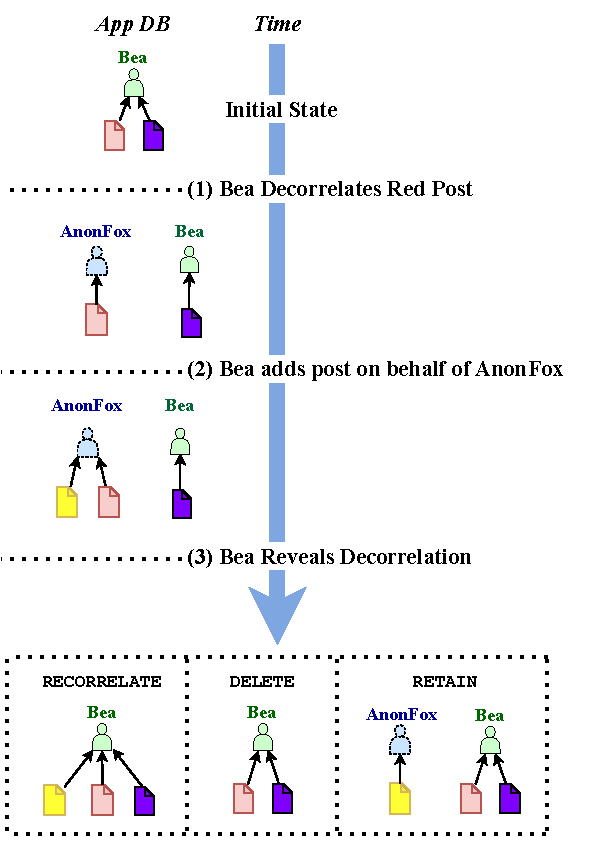
\includegraphics[width=.7\textwidth]{figs/ppreveal_policies}
    \caption[\texttt{RECORRELATE}, \texttt{DELETE}, and
    \texttt{RETAIN} policies maintain referential integrity for objects added
    after disguising that refer to a pseudoprincipal during reveal.]{After Bea
    decorrelates a story (red) to a pseudoprincipal, AnonFox, Bea or the
    application may add new stories that reference AnonFox (yellow). When Bea
    reveals and recorrelates to AnonFox, developers can
    choose to \texttt{RECORRELATE}, \texttt{DELETE}, or \texttt{RETAIN} any new
    content (\ie the yellow story) referring to AnonFox.}
\label{f:ppreveal}
\end{figure}

%
\sys identifies and accesses the disguised data to reveal using the user's
identifier \texttt{u}, their reveal credentials \texttt{cred}, and the disguise
identifier \texttt{d}.  The developer again provides a schema with annotated
foreign key relationships (\texttt{schema}). This allows \sys to perform checks
for referential integrity prior to reveal (\eg \sys will not restore removed
data that introduces a dangling reference) and recorrelate data from
pseudoprincipals to their original principal owner. 
%

\sys also requires the developer to specify a \emph{pseudoprincipal reference policy}
\texttt{pp\_ref\_policy} because pseudoprincipals may acquire new references
from application objects inserted after the time of disguise---for example, a
decorrelated comment might have new responses. To ensure that revealing a
decorrelate operation---which deletes pseudoprincipals---preserves referential
integrity, developers inform \sys how to, during reveal, handle these objects
added after disguising that refer pseudoprincipals of the disguise.
%

%
Developers choose between three options for pseudoprincipal-referring objects:
\one{} change the object's reference to point to the original principal
(\texttt{RECORRELATE}); \two{} delete the object (\texttt{DELETE}); or \three{}
continue referring to the pseudoprincipal (\texttt{RETAIN}).
Figure~\ref{f:ppreveal} demonstrates the result of each policy when revealing a
story added to Bea's pseudoprincipal after a decorrelation disguise.
%
This option applies to all rows to reveal; another choice of API could support a
menu of options, such as per-table checks and fixes (where the developer
specifies per-table policies) or per-inserted-object ones (where the developer
makes application modifications to log all added references to
pseudoprincipals).
%

%
\sys uses the developer-provided \texttt{allow\_partial\_row\_reveal} flag to
determine whether \sys can partially reveal a row (\ie restore some modified
columns even when unable to reveal others). 
%
Partial row reveals occur because \sys only reveals a modified column if the
current column value of the row in the application database matches the value
generated by the modify operation during the disguise
(\S\ref{s:semantics:spec}). This stops \sys from overwriting application changes
to modified columns. 
%

%
\subsection{\texttt{CanSpeakFor}}
\label{s:semantics:speakfor}
    \texttt{CanSpeakFor} lets an application allow a user \texttt{u} to prove to
    the application that they have the authority to speak-for any principal
    stemming from a (potentially recursive) decorrelation of \texttt{u}. The
    application can then use this authorization to, for example, allow the user
    to edit their pseudoprincipals' data.
    
    \texttt{CanSpeakFor} returns a list of all user IDs of principals that
    \texttt{u} can speak-for.

\begin{center}
    \begin{longtable}{|m{0.12\textwidth}|m{0.81\textwidth}|}
        \hline
        \textbf{Argument} & \textbf{Description} \\
        \hline
             \texttt{u}& The user's unique identifier. \\
        \hline
             \texttt{cred}& The user's reveal credentials (their password, private key, or
    backup token).\\
        \hline
    \end{longtable}
    \end{center}
    \vspace{-24pt}
   
    \sys identifies and accesses all of \texttt{u}'s speaks-for records making
    up \texttt{u}'s speaks-for chain using the user's identifier \texttt{u} and
    their reveal credentials \texttt{cred}.

\subsection{\texttt{RecordUpdate}}
\label{s:semantics:updates}

\texttt{RecordUpdate} enables a developer to update disguised data prior to
revealing it, in order to reflect global database changes (\eg schema migrations)
applied since the time of disguise.
%
Invoking \texttt{RecordUpdate} timestamps and logs a developer-provided update
specification---a data transformation function---to reflect a global update
performed on undisguised data. All updates since the time of disguise will be
performed in chronological order on disguised data prior to revealing it.

\texttt{RecordUpdate} returns \texttt{true} on successful recording in \sys's
    log, and \texttt{false} on failure.

\begin{center}
    \begin{longtable}{|m{0.18\textwidth}|m{0.75\textwidth}|}
        \hline
        \textbf{Argument} & \textbf{Description} \\
        \hline
             \texttt{update\_spec}& a reveal-time update specification reflecting
    the data transformations performed on table rows. The specification maps a
    set of table rows to a set of updated table rows.\\
        \hline
    \end{longtable}
    \end{center}
    \vspace{-24pt}

%
    \sys expects \texttt{update\_spec} to take a user's disguised data rows and
    produce updated versions of disguised data rows.
%
    Oftentimes, these updates may be a subroutine of the global database update. 
%
    For example, if a developer wants to normalize all URLs in Lobsters
    \texttt{stories}, they might first read all stories, then normalize the URL
    in each story individually, and finally \texttt{INSERT...UPDATE} the
    normalized stories. 
%
    An update specification given to \sys could just capture the normalization
    step, producing normalized URL stories for the stories in a user's disguised
    data.
%

%
    In other situations, no such subroutine of the global update exists because
    the global update uses queries that apply to entire database tables instead
    of rows.  In these scenarios, the developer must write a separate update
    specification for updating disguised data rows.
%
    For example, Lobsters has a schema migration that adds a column to the
    \texttt{users} table.  The global update performs an \texttt{ALTER TABLE}
    query, while the update specification given to \sys receives user rows
    without the column as input, and outputs user rows with the column.
%

\sys supports as update specifications any pure functions without side effects,
and which execute deterministically in their input (placeholder or disguised
rows).
%
For all other update specifications, \sys assumes that any nondeterminism or side effects from performing the
    update will maintain application correctness.
    %

%
    To exemplify an unsupported update, take a global update that calculates the
    current vote count of a story to store as a story's \texttt{vote\_count}
    attribute. 
%
    This update thus depends on other disguised rows, namely \texttt{vote} rows.
%
    If a disguise has removed both a user's story and its votes, then when \sys
    reveals the disguise, \sys will first reveal disguised stories before
    revealing disguised votes in order to maintain referential integrity. 
%
    But when applying a \texttt{vote\_count} update specification to stories,
    \sys will find 0 votes for all of them, because their votes have not yet
    been restored.
%
    \sys supports this update only if this 0-vote state counts as correct
    application behavior.
%

    
\subsection{\sys's API Without Encryption}
\label{s:noencrypt-api}
A subset of Edna's API suffices to provide the same semantics for disguises
without encryption. Users do not need to register with \sys; applications can
use normal user authentication to authorize revealing; disguising
already-disguised data no longer requires a user's reveal credentials; and
reveal-time updates can be applied immediately to disguised data instead of
logged and applied at reveal time.

%%%%%%%%%%%%%%%%%%%%%%%%%%%%%%%%%%%%%%%%%%%%%%%%%%%%%%%%%%%%%%%%%%%
\section{Disguise Specifications}
\label{s:semantics:spec}

\sys's API requires a developer to provide a disguise specification when
invoking \texttt{DisguiseData}, which describes the effects of a disguise (and
undone by a reveal).  As previously shown in Figure~\ref{f:spec}, each
specification operation consists of the disguise operation type, the database
table name, and a SQL \fn{WHERE} predicate.
%

%
A disguise is invoked either automatically by the application, or by a specific
user of the application identified by their user ID (\texttt{u\_opt =
Some(uid)}).
% 
If not invoked by a specific user, the disguise applies to all data matching the
disguise specification's predicate.
%
If a disguise is user-specific, then only data that has a foreign key to that
user's identifier (is ``owned'' by that user) and matches the disguise
specification's predicate will be disguised. Invoking a disguise with
\texttt{u\_opt = Some(uid)} will thus add a condition on a disjunction of
"\texttt{[fk\_col] = [uid]}" clauses for all foreign keys \texttt{fk\_col} to
the application's principals table. For example, a predicate of \texttt{WHERE
true} to disguise all data of a table will turn into \texttt{WHERE true AND
(author1 = uid OR author2 = uid)}.

\sys handles each disguise operation type as follows:
%

\paragraph{\texttt{REMOVE(table, pred)}.}
A remove operation removes the entire row that matches the operation's
predicate.
%
Developers should take care to handle referential integrity to removed rows, as
\sys will not cascade-delete referencing rows or introduce placeholders.
(Developers should instead use decorrelate operations to remove principal rows
and replace them with pseudoprincipals).
%

%
A reveal of a remove operation will reinsert all removed rows, unless
reinserting the row will violate a primary key or uniqueness constraint of the
application.
%

%
\paragraph{\texttt{MODIFY(table, column, modification\_pol, pred)}.}
A modify operation works at per-col\-umn granularity, and requires developers to
specify a modification policy for each column to modify in addition to the table
name and predicate.
%
The modification policy informs \sys how to generate new placeholder values for
each column to modify using one of \sys's value generation policies. The current
prototype supports constants (\eg "removed"), random values (\eg a random email
address), and values derived from the prior value (\eg a redacted phone number
with only area code visible).
%

%
Revealing a modify operation restores a row's column back to its state prior
to the disguise \emph{only if} the current column value matches the value
generated by the modify operation during the disguise. This prevents a reveal
from overwriting application changes to the column value since the time of
disguise.
%
Some rows may thus end up partially revealed, with only some modified columns
restored back to the original pre-disguise state.  Developers can set the
\texttt{allow\_partial\_row\_reveal} flag to \texttt{false} when invoking
\texttt{RevealData} to disable partial row reveals. This will prevent \sys from
revealing any column values in a row with at least one conflicting column value.
%

%
\paragraph{\texttt{DECORRELATE(table, fk\_keys, group\_by, pred)}.}
%
A decorrelate operation requires developers to additionally specify which
foreign keys for the table rows to rewrite, and a \texttt{group\_by} attribute
if rows with the same value for that attribute should refer to the same
pseudoprincipal after decorrelation.
%
A decorrelate operation only applies to rows with foreign key relationships to
the principals table (if specified on other foreign keys, the operation will do
nothing).
%
Developers also provide a principal-generation policy
(\texttt{principal\_gen}) to \texttt{DisguiseData} using \sys's value generation
policies to tell \sys how to generate a pseudoprincipal row.
%

%
If the application invokes \texttt{DisguiseData} with \texttt{u\_opt =
Some(uid)}, then \sys only decorrelates the specified foreign key attributes
that refer to \texttt{uid} (for rows that match the predicate). 
%
Otherwise, the disguise applies over all users and \sys decorrelates all
specified foreign keys for all rows matching the predicate.
%

%
For all rows to decorrelate with the same \texttt{group\_by} attribute value,
\sys rewrites the foreign keys to decorrelate to the same randomly generated
pseudoprincipal.
%
If no \texttt{group\_by} attribute is specified, each row gets a unique
pseudoprincipal.
%
Thus, no two disguises share the same pseudoprincipals, and no two tables share
the same pseudoprincipals.
%

\section{Example}
 \label{s:semantics:example}  
%
\begin{figure}
    \centering
    \begin{subfigure}[t]{.47\columnwidth}
    \centering
    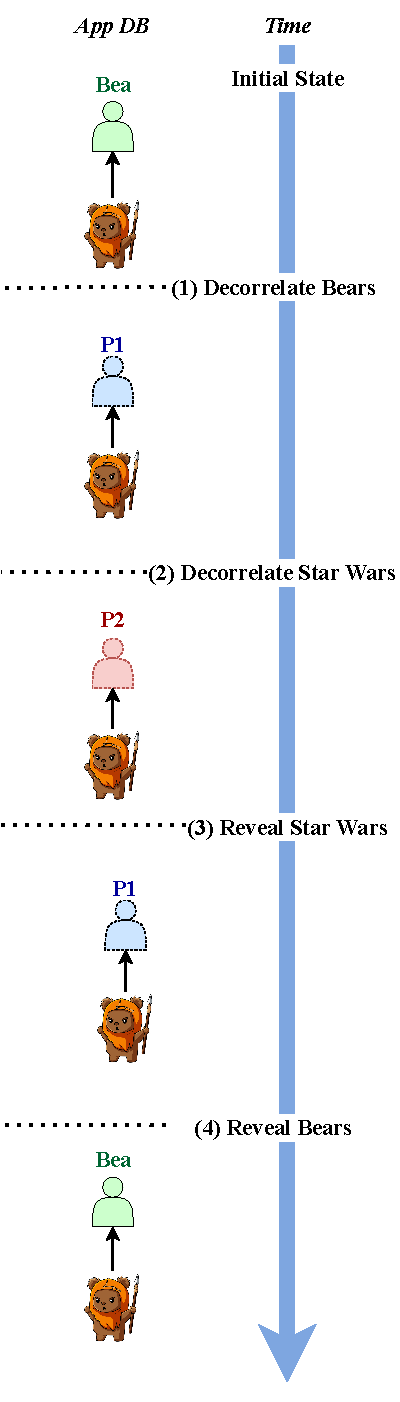
\includegraphics[width=.75\textwidth]{figs/composition-hl-inorder}
  \caption{Bea's reveal of ``Star Wars'' stories keeps ``Ewok'' stories still
        decorrelated under the ``bears'' disguise. Only after revealing
        ``bears'' stories does \sys restore ownership back to Bea.}
    \label{f:composition-hl-inorder}
    \end{subfigure}
    \hfill
\begin{subfigure}[t]{.47\columnwidth}
    \centering
    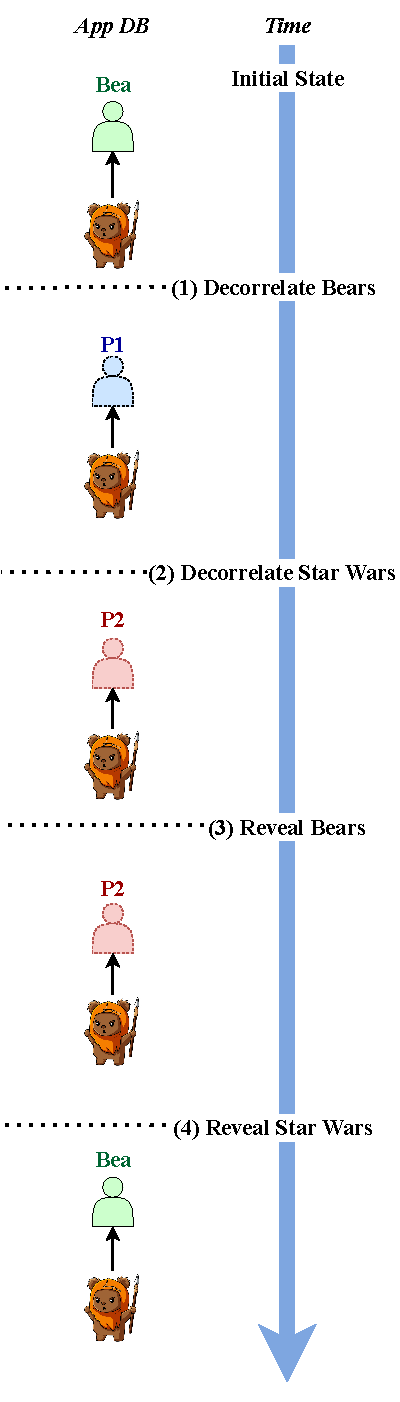
\includegraphics[width=.75\textwidth]{figs/composition-hl-ooo}
  \caption{Bea's reveal of ``bears'' stories keeps ``Ewok'' stories still
    decorrelated under the ``Star Wars'' disguise, which was applied after
    disguising ``bears''. Only after revealing ``Star Wars'' stories does \sys
    restore ownership back to Bea.}
\label{f:composition-hl-ooo}
\end{subfigure}
    \caption[\sys only reveals the original state of data disguised multiple times once
    all disguises applied to the data have been revealed.]{
        If Bea decorrelates an ``Ewok'' story twice---once via a ``bears''
        disguise, and once via a ``Star Wars'' disguise---\sys only recorrelates
        the story back to Bea once Bea reveals \emph{both} disguises.}
\label{f:composition-hl}
\end{figure}

%
To illustrate use of \sys's API and semantics, this example revisits the disguise 
specification for Lobsters topic-based anonymization (Figure~\ref{f:spec}). 
Figure~\ref{f:composition-hl} illustrates the various steps a user Bea would
take to apply the disguise for two topics, ``bears'' and ``Star Wars''.

\begin{enumerate}[nosep]
    \item[0)] Initially, the application starts out with Bea registered as an
        \sys principal via a call to \texttt{RegisterPrincipal} with Bea's
        password and keypair. Bea owns one story, with topic ``Ewoks''.

    \item[(1)] Bea invokes the application to decorrelate all ``bears'' stories 
        from their account: 

            \vspace{12pt}
            \begin{lstlisting}[style=rust,escapeinside={(*}{*)}]
                let did_bears = DisguiseData(
                    u_opt: Some("Bea"), 
                    spec: topic_anon_spec[Tag="bears"],
                    principal_gen: global_pp_generator,
                    schema: global_schema,
                    disguise_over: None)
            \end{lstlisting}

        This causes the application to instantiate the
        topic-based anonymization disguise specification with tag ``bears''.
        \sys rewrites the \texttt{author} foreign key values of ``bears''
         stories---which include Bea's ``Ewok'' story---to refer to generated
        pseudoprincipal $P_1$.

        \item[(2)] Bea invokes the application to decorrelate all ``Star Wars''
            stories from
        their account: 

        \vspace{12pt}
        \begin{lstlisting}[style=rust,escapeinside={(*}{*)}]
            let did_star_wars = DisguiseData(
                u_opt: Some("Bea"), 
                spec: topic_anon_spec[Tag="Star Wars"],
                principal_gen: global_pp_generator,
                schema: global_schema,
                disguise_over: Some("bea_password"))
        \end{lstlisting}

        This again causes the application to instantiate the topic-based
        anonymization disguise specification with tag ``Star Wars''. Bea also
        provides reveal credentials (\eg their password) so that any of their existing
        disguised stories can be disguised again. \sys rewrites the
        \texttt{author} foreign key values of ``Star Wars'' stories---again
        including Bea's ``Ewok''' story---to generated pseudoprincipal $P_2$.
    
    \item[(3)] Bea next reveals one of their disguises:
        \vspace{12pt}
        \begin{lstlisting}[style=rust,escapeinside={(*}{*)}]
            RevealData(
                u: "Bea", 
                cred: "bea_password",
                d: did_bears,  // or did_star_wars
                pp_ref_policy: RECORRELATE,
                allow_partial_row_reveal: true,
                schema: global_schema)
        \end{lstlisting}

        After reveal, any unrevealed disguises remain applied to the ``Ewoks''
        story.
        %
        This means the story will remain decorrelated to $P_1$ even if the ``Star
        Wars'' disguise decorrelating to $P_2$ is revealed
        (Figure~\ref{f:composition-hl-inorder}).
    %
        And if only the ``bears'' 'disguise decorrelating to $P_1$ were
        revealed, but not the ``bears'' disguise, the data would remain
        decorrelated to $P_2$.  (Figure~\ref{f:composition-hl-ooo}).

    \item[(4)] Finally Bea reveals the remaining disguise applied to ``Ewok''
        stories:

        \vspace{12pt}
        \begin{lstlisting}[style=rust,escapeinside={(*}{*)}]
            RevealData(
                u: "Bea", 
                cred: "bea_password",
                d: did_star_wars,  // or did_bears
                pp_ref_policy: RECORRELATE,
                allow_partial_row_reveal: true,
                schema: global_schema)
        \end{lstlisting}
        
        This restores ownership of the story back to Bea's account.

\end{enumerate}

%%%%%%%%%%%%%%%%%%%%%%%%%%%%%%%%%%%%%%%%%%%%%%%%%%%%%%%%%%%%%%%%%%%

\section{Disguise Composition}
\label{s:semantics:hl:composition}

As shown in \S\ref{s:semantics:example}'s example, multiple disguises can apply
to a user's data. The example demonstrates how Bea can disguise their data
multiple times; however, a user with access to all data (\eg an application
admin) could also decide to apply multiple global disguises to all user data,
including Bea's.  In this second case, disguises apply to all data satisfying
the disguise specification's predicates regardless of which user owns the data,
and disguise composition is straightforward (updating the already-disguised
data).

In the first case, however, when the application invokes \texttt{DisguiseData}
on behalf of Bea (\texttt{u\_opt = Some("Bea")}), \sys disguises only data
associated via a foreign key to Bea's application principal.
%
This means that if a user like Bea wishes to disguise already-decorrelated data
multiple times, \sys must have the user's reveal credentials
(\texttt{disguise\_over = Some(cred)}). This allows \sys to access Bea's
correlations to pseudoprincipals in order to disguise their pseudoprincipals'
data.
%
\sys will then treat all of the user's pseudoprincipals' data as if they belong
to the user themselves, and---depending on the disguise specification---will
remove, modify, or create a new pseudoprincipal owner for these
pseudoprincipals' data.
%
\S\ref{s:composition} fleshes out \sys's design for disguise composition when
a user has already decorrelated some of their data.

%
To reveal their data back to its original state, a user must reveal all
disguises composed atop the data.
%

%%%%%%%%%%%%%%%%%%%%%%%%%%%%%%%%%%%%%%%%%%%%%%%%%%%%%%%%%%%%%%%%%%%
\section{Shared Data}
Many applications support shared data; in Lobsters, for example, messages
between users are owned by both users.
%or co-authored papers in HotCRP.
%
\sys's default semantics for shared data implement an ownership model inspired
by a common treatment of shared data as jointly owned.
%
When a user's disguise removes shared data, \sys decorrelates the data from the
\xxing user, but preserves the data and its association with other owners.
%
\sys removes the data once all users have \xxed it and all ownership links are
to pseudoprincipals.
%
Any owner can reveal the message, which restores the message to the database if
it does not exist, and recorrelates only the revealing user; all disguised
owners remain decorrelated as pseudoprincipals until they also choose to reveal
the message.
%
Regardless of the reveal order, if all owners reveal the message, \sys returns
the message to its original state.
%

%
For each shared data object, each owner has an associated unique
pseudoprincipal. If only some owners have disguised the row, the row will refer
to the disguised owners' unique pseudoprincipals' identifiers instead of the
owners'.
%
When a user reveals a shared data row, all users still disguised remain
associated with their unique pseudoprincipal (which can be reused over multiple
remove disguises).
%

\begin{figure}
    \centering
    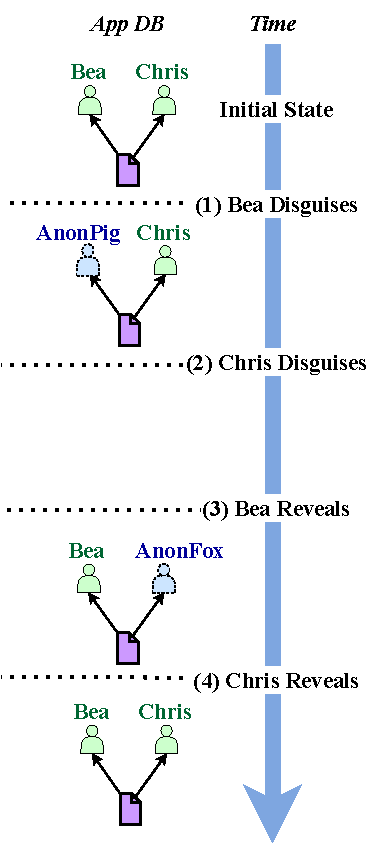
\includegraphics[width=.4\textwidth]{figs/shared_hl}
    \caption[\sys supports joint ownership semantics when disguising shared data.]{\sys supports joint ownership semantics, where shared data is not
    removed until all users have disguised their accounts. Owners can return in
    any order, and the message remains decorrelated from unrevealed owners.}
\label{f:shared:hl}
\end{figure}

%
For instance, consider the scenario in Figure~\ref{f:shared:hl} where Bea and
Chris share a Lobsters message. Bea maps to unique pseudoprincipal AnonPig for this
shared message, and Chris to AnonFox.
\begin{enumerate}[nosep]
    \item[(1)] When Bea \xxs the message, the message is owned by
Chris and a pseudoprincipal;
    \item[(2)] If Chris then \xxs the message, \sys removes it.
    \item[(3)] If Bea reveals the message, this restores the message to the database
and recorrelates only Bea; Chris remains decorrelated as a pseudoprincipal.
\item[(4)] When Chris reveals the message, \sys returns
the message to its original state.
\end{enumerate}
%

\S\ref{s:design:shared} dives deeper in how \sys's design achieves these shared
data semantics.

%%%%%%%%%%%%%%%%%%%%%%%%%%%%%%%%%%%%%%%%%%%%%%%%%%%%%%%%%%%%%%%%%%%

